\documentclass[]{article}
\usepackage{lmodern}
\usepackage{amssymb,amsmath}
\usepackage[utf8]{inputenc} 
\usepackage{ifxetex,ifluatex}
\usepackage{graphicx}
\usepackage{fixltx2e} % provides \textsubscript
\ifnum 0\ifxetex 1\fi\ifluatex 1\fi=0 % if pdftex
  \usepackage[T1]{fontenc}
  \usepackage[utf8]{inputenc}
  \usepackage{eurosym}
\else % if luatex or xelatex
  \ifxetex
    \usepackage{mathspec}
    \usepackage{xltxtra,xunicode}
  \else
    \usepackage{fontspec}
  \fi
  \defaultfontfeatures{Mapping=tex-text,Scale=MatchLowercase}
  \newcommand{\euro}{€}
\fi
% use upquote if available, for straight quotes in verbatim environments
\IfFileExists{upquote.sty}{\usepackage{upquote}}{}
% use microtype if available
\IfFileExists{microtype.sty}{%
\usepackage{microtype}
\UseMicrotypeSet[protrusion]{basicmath} % disable protrusion for tt fonts
}{}
\ifxetex
  \usepackage[setpagesize=false, % page size defined by xetex
              unicode=false, % unicode breaks when used with xetex
              xetex]{hyperref}
\else
  \usepackage[unicode=true]{hyperref}
\fi
\hypersetup{breaklinks=true,
            bookmarks=true,
            pdfauthor={},
            pdftitle={},
            colorlinks=true,
            citecolor=blue,
            urlcolor=blue,
            linkcolor=magenta,
            pdfborder={0 0 0}}
\urlstyle{same}  % don't use monospace font for urls
\setlength{\parindent}{0pt}
\setlength{\parskip}{6pt plus 2pt minus 1pt}
\setlength{\emergencystretch}{3em}  % prevent overfull lines
\setcounter{secnumdepth}{0}

\date{}
\begin{document}
\title{Projet Programmation 2}
\author{Mathieu Seurin \\
Elias Rhouzlane}
\date{\today}
 
\maketitle
\begin{abstract}
Ce jeu de ‘SameGame’ est grandement inspiré par le mode 2 joueurs du jeu Pokemon Puzzle
Challenge sur GameBoy (\href{http://www.playr.org/play/pokemon_puzzle_challenge/1366}{Jouable ici})

Ainsi le jeu a été pensé dans ce sens et donc beaucoup de choix ont été fait en prévision de
l’implémentation des fonctionnalités du jeu d’origine. C’est pour cela que certains choix peuvent
sembler étranges ou inadaptés, mais c’était en prévision de l’implémentation de fonctionnalités plus
avancés.
\end{abstract}
\section*{Fonctionnement du jeu}
Deux joueurs s’affrontent, chacun avec son plateau composé de diverses cases de couleurs. Les
plateaux montent au fur et à mesure, de nouvelles lignes se rajoutent en bas. Une fois que le plateau
atteint le haut du jeu, c’est perdu. Pour éviter ça les joueurs disposent d’un swapper (curseur) qui
permet d’échanger deux cases. Lorsqu’au moins trois cases de la même couleur sont alignées
(horizontalement ou verticalement) on supprime ces cases, permettant ainsi de libérer le plateau
petit à petit. La montée du plateau est de plus en plus rapide, rendant ainsi l’affrontement de plus en
plus tendu. En plus de cette montée, si les joueurs arrivent à faire des combinaisons de plus de 3
couleurs, ils peuvent envoyer des mauvais blocks à leurs adversaires. Ces mauvais blocks occupent
plusieurs cases, ne peuvent être swappés, et ne sont pas désolidarisables. Le seul moyen de les
détruire est de faire une combinaison de trois couleurs juste à côté d’eux, les transformant ainsi en
cases de couleurs utilisables.
\pagebreak
\section*{Objectifs atteints}
\begin{itemize}
\itemsep5pt\parskip1pt\parsep0pt
\item 
Avoir un menu avec des effets simples
\item 
Avoir un moteur d’affichage permettant d’ajouter facilement de nouveau effets et de
nouveaux menus
\item
 Pourvoir générer des plateaux remplis de cases de couleurs
\item
 Pouvoir afficher deux plateaux jouables en parallèles
\item 
Pouvoir déplacer le curseur à l’écran, parcourir les cases, échanger les cases
\item 
Avoir un algorithme de suppression des cases alignées en ligne et colonne (pas de diagonale)
qui supprime en cas de chaine de plus de 3cases de même couleur
\item 
Pouvoir générer des mauvais blocks (‘bad’ block) qui sont composés de plusieurs cases
simples, censés vous bloquer puisqu’ils ne sont ni interchangeables (pas de swap) ni désolidarisables
\item 
Avoir un algorithme qui gère la gravité du plateau non seulement pour les cases simples mais
également pour les ‘bad’ blocks qui sont composés de cases simples ‘soudés’ entre elles, ainsi un
‘bad’ block ne peut tomber que si toutes les cases sous lui sont libres (non implémenté)
\item 
Générer des lignes de cases
\item 
Avoir un système de score
\item
Avoir un système d'affichage d'information pour chaque joueur
\item 
Fin de jeu, lorsque la ligne du haut est dépassé
\end{itemize}

\section*{Objectifs restants}
\begin{itemize}
\itemsep5pt\parskip1pt\parsep0pt
\item 
Pouvoir envoyer de mauvais blocks à l’adversaire à l’aide de combos
\item 
Quelques glitches d'animation à résoudre
\item 
Pouvoir sauvegarder, charger, continuer et mettre en pause une partie
\item
Améliorer le système d'affichage d'information et le rendre plus lisible
\item
Enregistrer les scores et faire un tableau des scores
\item 
Créer des modes histoire et en ligne en plus du mode arcade implémenté
\end{itemize}

\pagebreak
\section*{Choix divers}
\subsection*{Pourquoi une ``hidden row'' ?}

Le plateau est censé monter petit à petit et non pas par à-coup, ainsi on est censé voir la ligne du bas
se montrer petit à petit jusqu’à ce qu’elle soit active. Ainsi il fallait qu’elle soit déjà générée et
disponible pour pouvoir l’afficher (même si elle aurait été grisée pour montrer qu’elle n’est pas
encore active)
Ceci a pas mal de conséquences, notamment de lors des parcours de board, les indices commencent
souvent à 1 pour les lignes (row), bien qu’ils commencent à 0 pour les colonnes (col)

\subsection*{Les bad blocks}
Les bad blocks ont posés un problème car lors de leur implémentation nous avions déjà fait la plupart
des fonctions, notamment destruction, gravité et swap, il a donc fallu recoder ces fonctions pour
pouvoir gérer les Bad blocks, puisque ceux-ci ont un comportement assez particulier, bien différents
des simples cases de couleurs.
Comment gérer la gravité :
Il nous semblait plus simple d’appliquer la gravité sur tous les blocs, quitte à séparer les bad blocks,
puis reconstruire le bad block, plutôt que de gérer chaque cas, car il y a aurait eu beaucoup de
problème en cas de plusieurs bad block ou lorsque des cases se retrouvaient au-dessus d’un bad
block
\subsection*{Le passage aux Sprites}
Dans cette version certains objets visuels sont des sprites, on double quasiment les fps de ce fait car on ne regénère
pas tout le plateau à chaque tour de boucle.

\section*{Arbres d'héritage}
\subsection*{Window}
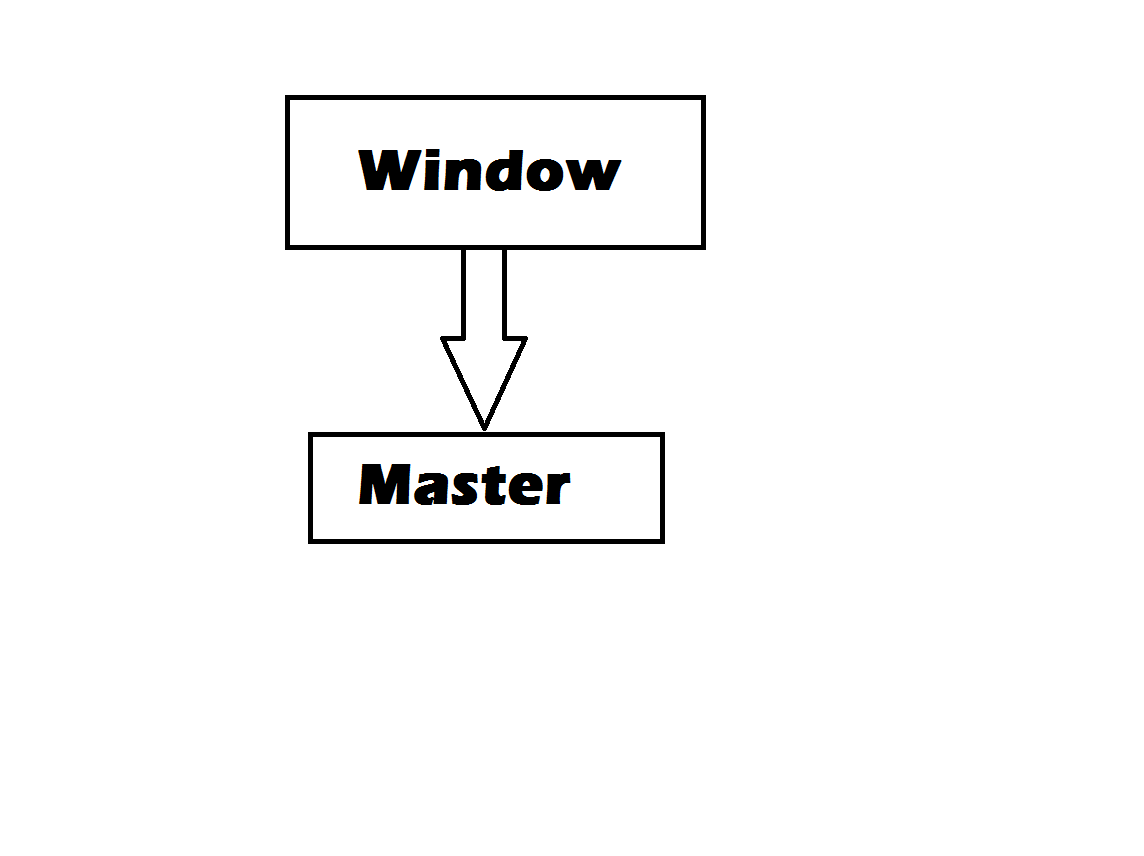
\includegraphics[width=13cm]{Window}
\subsection*{State}
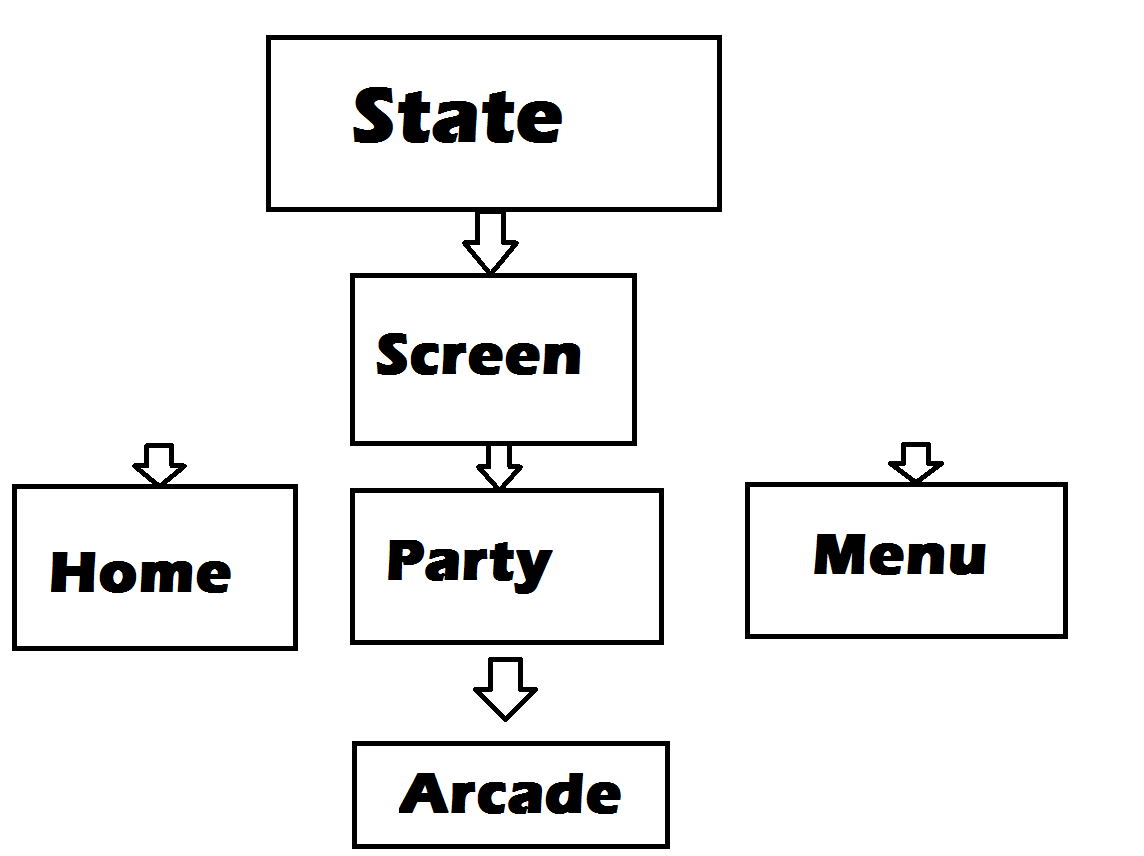
\includegraphics[width=13cm]{State}
\subsection*{Sprite}
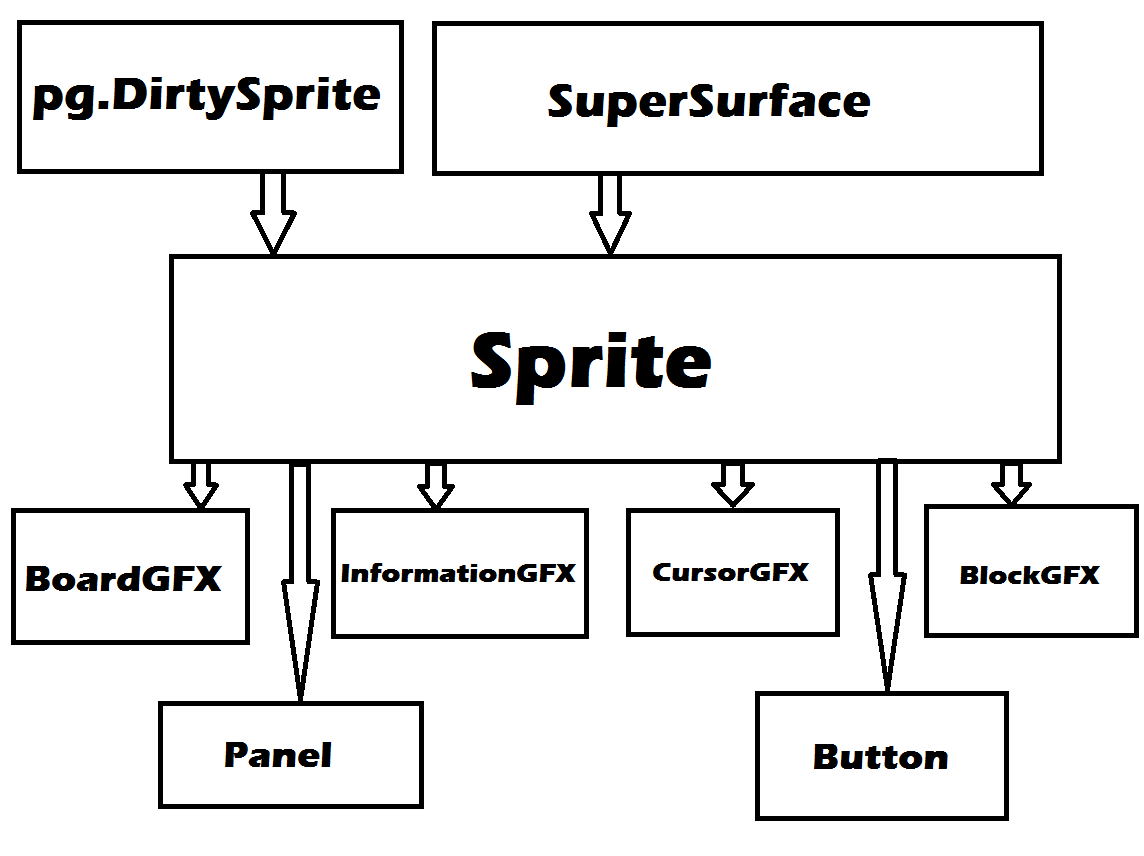
\includegraphics[width=13cm]{Sprite}
\subsection*{Effect}
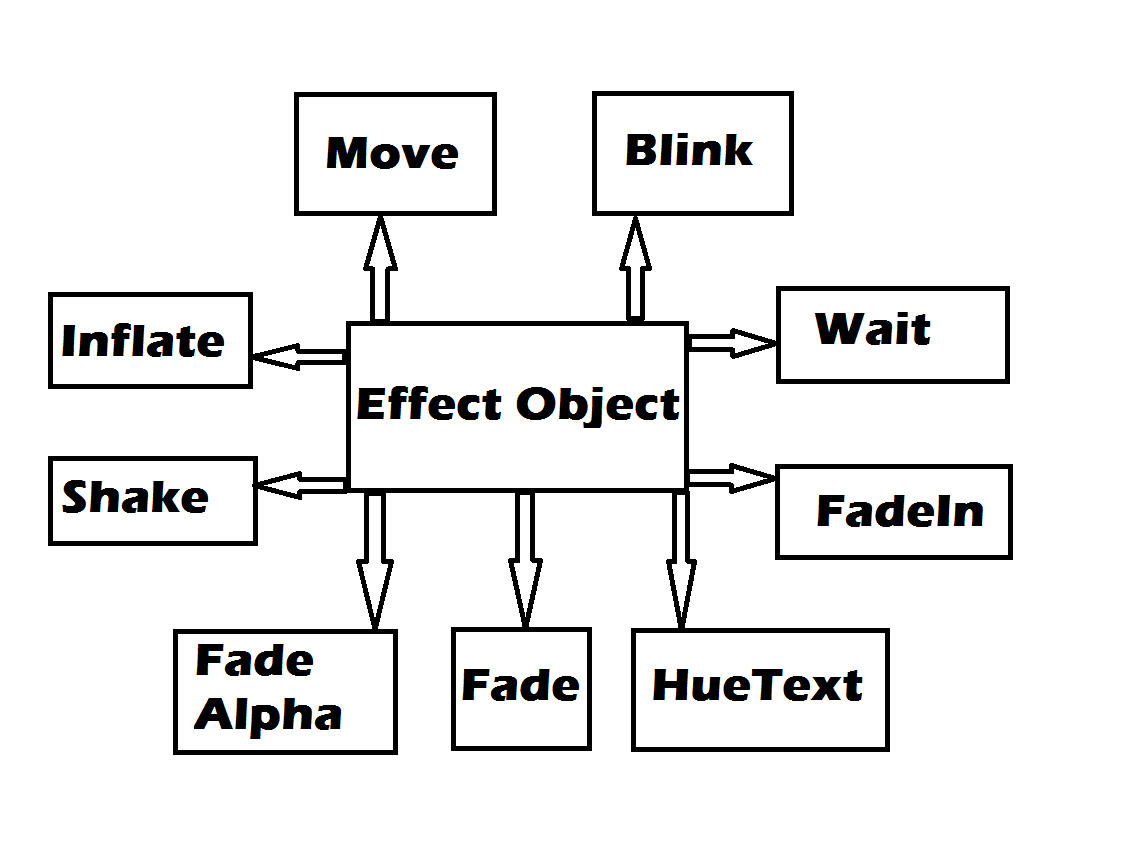
\includegraphics[width=13cm]{Effect}
\subsection*{PlayerInformation}
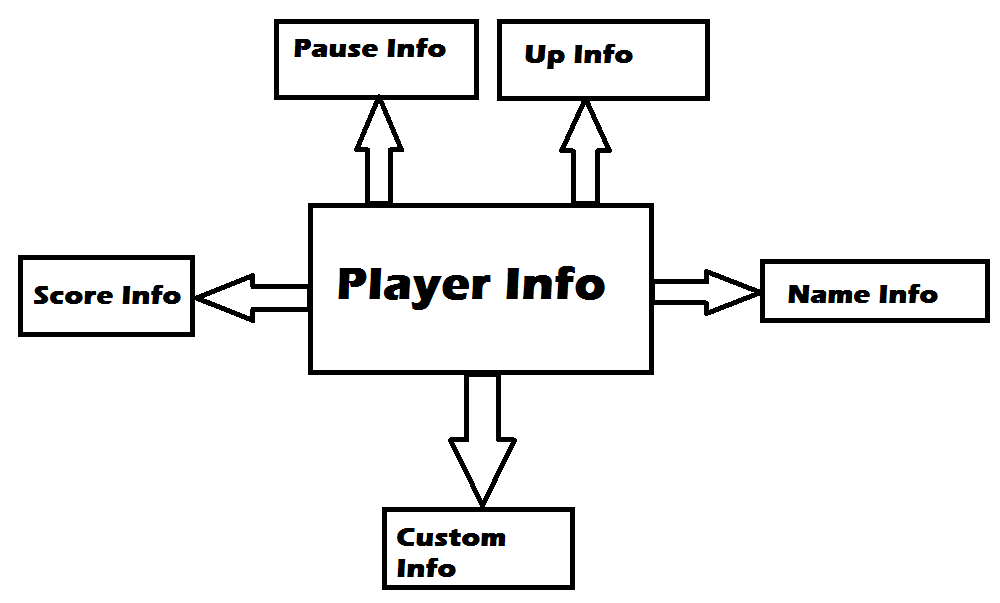
\includegraphics[width=13cm]{PlayerInformation}
\end{document}
